\section{Divisione efficiente}
L' algoritmo usato precedentemente non risulta molto efficiente e soprattutto non è in tempo costante.
Un algoritmo migliore sarebbe quello che si vede alle elementari: la divisione in colonna.
Supponiamo di dover dividere 19374 per 171:
\begin{itemize}
    \item si prendono le prime 3 cifre del dividendo: 193 e si controlla quante volte entri nel divisore 171, in questo caso entra 1 volta
    
    \item il quoziente ha come prima cifra 1

    \item sottraggo 171 a 193 ed ottengo il primo resto
    
    \item abbasso la prossima cifra e ripeto il controllo e l' aggiornamento
\end{itemize}
Abbiamo alcuni problemi nello scegliere quante cifre prendere, se ne prendo poche ottengo 0 come cifra, in realtà va bene in quanto mi fornisce uno 0 in testa che fa parte del quoziente.
Inoltre in binario ci viene ancora più semplice la fase di comparazione in quanto un numero può entrare nell' altro solo 0 o 1 volte e per saperlo ci basta vedere quale dei due valori risulta maggiore dell' altro.

Supponiamo dunque di voler eseguire una divisione a 16 bit completa: $\frac{p}{q}$
\begin{itemize}
    \item $p$ a 16 bit
    \item $q$ a 16 bit
    \item $k$ quoziente può essere al massimo $\frac{65535}{1} = 65535$ che sta su 16 bit
\end{itemize}

Pongo il dividendo in due registri e lo estendo su 32 bit, per questo numero facciamo una estensione virtuale, nel senso che non usiamo registri per mantenere in memoria gli zeri più significativi.
Il divisore invece lo poniamo nella parte alta di 4 registri, quindi anche lui rappresentato su 32 bit.
La situazione iniziale deve quindi essere:
\begin{figure}[H]
    \centering
    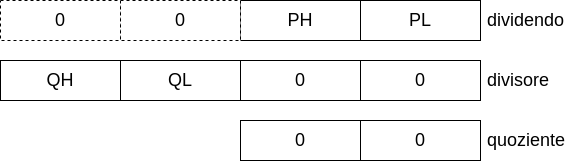
\includegraphics[width=250px]{images/12_Divisione_efficiente/divisione_fast.png}
\end{figure}

Ad ogni iterazione devo quindi vedere se $P > Q$, in tal caso ottengo 1, altrimenti 0:
\begin{itemize}
    \item se ottengo 1 sottraggo
    \item se ottengo 0 non faccio niente
\end{itemize}
alla fine shifto a destra Q.
Per collezionare le singole cifre le inserisco da destra all' interno del quoziente poi shifto a sinistra per farle andare al loro posto.
Si noti che la parte alta di P contiene degli zeri, quindi per i primi elementi il controllo si limita a vedere se la parte alta di Q è diversa da 0, per la parte bassa invece occorre un vera comparazione.
Dopo un po' di giri P e Q saranno allineati e quindi inizierò ad ottenere le vere cifre del quoziente.

L' algoritmo viene iterato per 16 volte, per non sprecare un registro inserisco un bit ad 1 come primo bit del quoziente, quando lo vedo comparire nel carry dopo gli shift so che ho fatto tutte le iterazioni necessarie.

Mappiamo i seguenti registri:
\begin{figure}[H]
    \centering
    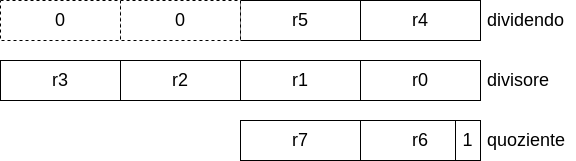
\includegraphics[width=250px]{images/12_Divisione_efficiente/divisione_fast_registri.png}
\end{figure}

\begin{verbatim}
    ; PARAMS
    ; r3:r2 divisore
    ; r5:r4 dividendo

    ; RETURN
    ; r5:r4 resto
    ; r7:r6 quoziente

    div16:
        ; controllo che non mi sia stato
        ; chiesto di dividere per 0
        mov r8, r2
        or r8, r3
        brne nodiv0

        ; in tal caso setto il carry come errore
        ; ed esco
        sec
        ret

        ; eseguo la vera divisione
    nodiv0:
        ; configuro i registri
        clr r0
        clr r1
        clr r6
        inc r6  ; inserisco 1 come LSB
        clr r7
        clr r8
        
    divstart:
        ; shift del divisore
        lsr r3  ; LSB va in carry
        ror r2  ; il carry va in MSB, LSB va in carry
        ror r1  ; il carry va in MSB, LSB va in carry
        ror r0  ; il carry va in MSB, LSB va in carry
        
        tst r3
        brne nosub
            ; se è diverso da 0 non devo sottrarre
        tst r2
        brne nosub
            ; se è diverso da 0 non devo sottrarre

        cp r5,r1
        brcs nosub
            ; r5 < r1 ho 0 e non devo sottrarre
        brne oksub
            ; r5 > r1 ho 1 e devo sottrarre 
            ; r5 == r1 devo controllare l'ultimo byte
        cp r4,r0
        brcs nosub
            ; r4 < r0 ho 0 e non devo sottrarre
            ; r4 >= r0 ho 1 e devo sottrarre
        
    oksub:
        ; eseguo la sottrazione
        sub r4,r0
        sbc r5,r1
        sec         ; setto il carry per inserire 1
        rjmp div1
        
    nosub:
        clc         ; pulisco il carry per inserire 0
        
    div1:
        rol r6
        rol r7
        brcc divstart
            ; se carry = 1 ho finito le iterazioni
        
    divfine:
        clc     ; divisionre corretta quindi carry = 0
        ret
\end{verbatim}

